\chapter{Integration}
In mathematics we are often given a function $f$ and asked to find a function $F$ whose derivative is $f$. $\;F$ in this situation is called the integral of $f$. 
It is usual to develop a list of integrals by differentiating a range of functions then using those to work backwards. The terms integration and anti-differentiation are synonymous. Generally we will use the term integration, however, both are acceptable.

\textbf{Examples}
\begin{enumerate}
\item Because $y =x^{2}$ gives $y^{ \prime } =2 x$ we can say that an integral of $2 x$ is $x^{2}$. 

\item Because $y =x^{2} +1$ gives $y^{ \prime } =2 x$ we can say that another integral of $2 x$ is $x^{2} +1$. 

\item Because $y =x^{2} +c$ where $c$ is a constant gives $y^{ \prime } =2 x$ we can say that an integral of $2 x$ is $x^{2} +c$. 

\item Because $y =e^{x}$ gives $y^{ \prime } =e^{x}$ we can say that an integral of $e^{x}$ is $e^{x}$. In fact we say that the integrals of $e^{x}$ are $e^{x} +c$ where $c$ is a constant. 

\item Because $y =\ln  x +c$ where $c$ is a constant gives $y^{ \prime } =\frac{1}{x}$ we can say that a family of integrals of $\frac{1}{x}$ is $\ln  x +c$. This is often written $\ln  k x$ where $c =\ln  k$ is the constant 

\item This can be generalised. $y =\ln  \left \vert x\right \vert  +c$ also gives $y^{ \prime } =\frac{1}{x}$ so in general the integrals of $\frac{1}{x}$ are $\ln  \left \vert x\right \vert  +c$. \end{enumerate}


\section{Rules of Integration}
The examples shown above begin the process of establishing the start of a list of integration rules. It
is not the intention here to list all of the rules that are required however at this stage let us explore the Power Rule to establish a rule for antedifferentiating
an expression of the form $y =x^{n}$ 

\bigskip 
\begin{tabular}[c]{|l|l|}\hline
$f$  & $f^{ \prime }$  \\
\hline
$x$  & $1$  \\
\hline
$x^{2}$  & $2 x$  \\
\hline
$x^{3}$  & $3 x^{2}$  \\
\hline
$x^{4}$  & $4 x^{3}$  \\
\hline
\end{tabular}\ or
\
\begin{tabular}[c]{|l|l|}\hline
$f$  & $f^{ \prime }$  \\
\hline
$x$  & $1$  \\
\hline
$\frac{1}{2} x^{2}$  & $x$  \\
\hline
$\frac{1}{3} x^{3}$  & $x^{2}$  \\
\hline
$\frac{1}{4} x^{4}$  & $x^{3}$  \\
\hline
\end{tabular}\ so
we can say \
\begin{tabular}[c]{|l|l|}\hline
$f^{ \prime }$  & $f$  \\
\hline
$1$  & $x +c$  \\
\hline
$x$  & $\frac{1}{2} x^{2} +c$  \\
\hline
$x^{2}$  & $\frac{1}{3} x^{3} +c$  \\
\hline
$x^{3}$  & $\frac{1}{4} x^{4} +c$  \\
\hline
\end{tabular}\ or
\
\begin{tabular}[c]{|l|l|}\hline
$f$  & $F$  \\
\hline
$1$  & $x +c$  \\
\hline
$x$  & $\frac{1}{2} x^{2} +c$  \\
\hline
$x^{2}$  & $\frac{1}{3} x^{3} +c$  \\
\hline
$x^{3}$  & $\frac{1}{4} x^{4} +c$  \\
\hline
\end{tabular}

\bigskip This establishes the pattern and if you think about the rule for differentiating $y =x^{n}$ you can soon establish the rule for antidifferentiating $x^{n}$.
\begin{equation*}\text{ Given a function }f (x) =x^{n}\text{ the integral of }f\text{is}\frac{x^{n +1}}{n +1} +c\text{ provided }n \neq  -1
\end{equation*}

\begin{equation*}\text{ If }f (x) =x^{ -1}\text{ then the integral of }f\text{ is }\ln  \left \vert x\right \vert  +c\text{ or }\ln  \left \vert k x\right \vert \text{ from above.}
\end{equation*}

All of the differentiation rules we have met so far
lead to integration rules. For instance we can establish rules for $\sin  x$, $\cos  x$, and $\sec ^{2} x\text{.}$ 

You will recall that we established also differentiation rules for adding, subtracting, multiplying
and dividing functions, for multiplying a function by a constant and for composite functions. The following
three rule for integration can be established from these. Other rules will follow later in the course.


 Let $F^{ \prime } =f$ , let $G^{ \prime } =g$ and let $c$ be a non-zero constant 

\textbf{Rule 1} 

The particular integral of $c f (x)$ is $c F (x)$ 

\textbf{Rule 2} 

The particular integral of $f (x) +g (x)$ is $F (x) +G (x)$ 

\textbf{Rule 3} 

The particular integral of $f (x) -g (x)$ is $F (x) -G (x)$ 

\subsection{Exercises 7.1.1}
\begin{enumerate}
\item Find the general integral of 


\begin{enumerate}
\item $f (x) =3$ 

\item $f (x) =3 x^{2} -2 x^{3}$ 

\item $f (x) =x^{\frac{2}{3}} -5 x^{ -\frac{1}{3}}$ 

\item $f (x) =\frac{1}{2 \sqrt{x}} +\frac{1}{\sqrt{2}}$ \end{enumerate}


\item Find $f (x)$ in each case. Give the general solution 


\begin{enumerate}
\item $f^{ \prime } (x) =5 x^{2}$. 

\item $f^{ \prime } (x) =1 -\frac{1}{x}$. \end{enumerate}


\item Find $f (x)$ given $f^{ \prime  \prime } (x) =6$. \end{enumerate}


Exercises 2 and 3 show examples of equations involving derivatives.
\ Any equation involving derivatives of a function is called a \emph{differential equation}.
\ We will look into this subject later in the course. 

\subsubsection{Supplementary Exercises}
Find the general integral in each case 


\columnsep =30pt
\begin {multicols}{3}
\begin{enumerate}
\item $4 x^{7}$ 

\item $10$ 

\item $\frac{8 x^{3}}{3}$ 

\item $3.2 e^{x}$ 

\item $\frac{1}{2 x}$ 

\item $\sqrt{x}$ 

\item $x^{1.2}$ 

\item $x^{\pi }$ 

\item $\frac{4}{\sqrt[{3}]{x^{4}}}$ 

\item $x^{ -\frac{2}{3}}$ 

\item $\left (2 x +1\right )^{2}$ 

\item $e^{x} +x^{e}$ 
\end{enumerate}
\end {multicols}
 

\section{Areas}
In this section we attempt to find the area under a curve. That is the area that lies between a curve
and the $x$-axis from $x =a$ to $x =b$. The area is bounded by the $x$-axis, a continuous curve $y =f (x)$ and the two vertical lines $x =a$ and $x =b$. 

When the region is bounded by straight lines the area is easy to find. For
example to find the area under the curve $y =x$ between $x =3$ and $x =5$ a simple diagram will lead to the conclusion that the area is $8$. 

When the area has curved sides the area is not so easy to find. Previously,
when we wanted to find the slope of a tangent line we found the slope of a secant line and applied the limiting process $\underset{h \rightarrow 0}{\lim }$. A similar procedure will be used to find the area. 

We first approximate
the area with rectangular strips then we take the limit of the areas of these rectangular strips by making the strips narrower and narrower and thus the
number of strips between $x =a$ and $x =b$ greater and greater. 

\subsubsection{Example}
Consider the curve $y =x^{2}$. Use rectangles to find the area under this curve between $0$ and $1$. 

Consider $4$ strips by constructing vertical lines at $x =\frac{1}{4}$, $x =\frac{1}{2}$, $x =\frac{3}{4}$ and $x =1$. Define the \emph{left sum} as the sum of the rectangles whose
left side is formed using $x =\frac{1}{4}$, $x =\frac{1}{2}$, $x =\frac{3}{4}$ and $x =1$. Define the \emph{right sum} as the sum of the rectangles whose
right side is formed by $x =\frac{1}{4}$, $x =\frac{1}{2}$, $x =\frac{3}{4}$ and $x =1$.
\begin{align*}\text{Left sum} &  = \frac{1}{4} \cdot 0^{2} +\frac{1}{4} \genfrac{(}{)}{}{}{1}{4}^{2} +\frac{1}{4} \genfrac{(}{)}{}{}{1}{2}^{2} +\frac{1}{4} \genfrac{(}{)}{}{}{3}{4}^{2} \\
 &  = 0 +\frac{1}{64} +\frac{1}{16} +\frac{9}{64} =\frac{1 +4 +9}{64} =\frac{7}{32} =0.21875 \\
\, &  &  \\
\text{Right sum} &  = \frac{1}{4} \genfrac{(}{)}{}{}{1}{4}^{2} +\frac{1}{4} \genfrac{(}{)}{}{}{1}{2}^{2} +\frac{1}{4} \genfrac{(}{)}{}{}{3}{4}^{2} +\frac{1}{4} \left (1\right )^{2} \\
 &  = \frac{1}{64} +\frac{1}{16} +\frac{9}{64} +\frac{1}{4} =\frac{1 +4 +9 +16}{64} =\frac{15}{32} =0.46875\end{align*}

It is clear from a diagram that the actual area is larger that the left sum and smaller than the
right sum.
\begin{equation*}0.21875 <A <0.46875
\end{equation*}

We could repeat this process with a larger number of strips but it is clear the process
would quickly become tedious. We can however simulate this process using Excel. 

\subsection{Riemann Sums}
For the curve $y =x^{2}$ set up a spreadsheet to show 10 strips or 20 strips or
30 strips etc. The following table gives the results you should obtain for a selection of numbers of strips

\begin{center}
\begin{tabular}[c]{|c|c|c|}\hline
$n$  & Left sum  & Right sum  \\
\hline
10
& 0.2850000  & 0.3850000  \\
\hline
20
& 0.3087500  & 0.3587500  \\
\hline
30
& 0.3168519  & 0.3501852  \\
\hline
100
& 0.3283500  & 0.3383500  \\
\hline
1000
& 0.3328335  & 0.3338335  \\
\hline
\end{tabular}\end{center}

It can be seen that a very accurate approximation to the area can be obtained as the number of rectangles increases. It
should be clear that as $n \rightarrow \infty $ both the left sum and the right sum approach the area under the curve 

We write
\begin{equation*}A =\underset{n \rightarrow \infty }{\lim }\text{Left sum} =\underset{n \rightarrow \infty }{\lim }\text{Right sum}
\end{equation*}

This process can be generalised by selecting any height within each rectangular strip
and finding the area of each strip using this height. Let there be $n$ strips and consider the $i^{t h}$ strip. Select a value of $x$ in the $i^{t h}$ strip call it $x_{i}$. The height of this rectangle will be $f (x_{i})$. Consider the situation described above where the area is bounded by the $x$-axis, a continuous curve $y =f (x)$ and the two vertical lines $x =a$ and $x =b$. 

With $n$ rectangles the length of the base of each rectangle is $ \Delta x =\frac{b -a}{n}$ 

The area of the $i^{t h}$ rectangle is $f (x_{i})  \Delta x$ 

The sum of all the rectangles is
\begin{equation*}\underset{i =1}{\sum ^{n}} f (x_{i})  \Delta x =f \left (x_{1}\right )  \Delta x +f \left (x_{2}\right )  \Delta x +\ldots  +f \left (x_{n}\right )  \Delta x
\end{equation*}

And
\begin{equation*}A =\underset{n \rightarrow \infty }{\lim }\left [\underset{i =1}{\sum ^{n}} f (x_{i})  \Delta x\right ]
\end{equation*}

If $f$ is a continuous function defined on the interval $\left [a ,b\right ]$ then as $n \rightarrow \infty $ the number represented by$\;\underset{i =1}{\sum ^{n}} f (x_{i})  \Delta x \rightarrow A$ the area under the curve $y =f (x)$. This number is called the definite integral of $f$ from $a$ to $b$ and is denoted by $\int _{a}^{b}f$ or $\int _{a}^{b}f (x) d x$
\begin{equation*}\int _{a}^{b}f (x) d x =\underset{n \rightarrow \infty }{\lim }\left [\underset{i =1}{\sum ^{n}} f (x_{i})  \Delta x\right ]
\end{equation*}

The expression $\underset{i =1}{\sum ^{n}} f (x_{i})  \Delta x$ is called a \emph{Riemann sum} after the German mathematician Bernard Riemann (1826-1866) who defined the integral
in this way. The symbol $\int $ was introduced by Leibniz and is called the \emph{integral sign}. 

\subsection{Exercises 7.2}
\begin{enumerate}
\item Evaluate $\int _{0}^{1}\sqrt{1 -x^{2}} d x$ by interpreting it as an area. 

\item Evaluate $\int _{0}^{3}4 d x$ by interpreting it as an area. 

\item Evaluate $\int _{0}^{3}\left (x +1\right ) d x$ by interpreting it as an area. 

\item Evaluate $\int _{0}^{3}\left (x -1\right ) d x$ by interpreting it as an area. \end{enumerate}


\section{Evaluating Definite Integrals}
The method of computing Riemann sums is often long and to achieve a result that is accurate enough requires a computer. Both Sir Isaac Newton
and Leibniz discovered a much simpler way based on the integral. This discovery is called \emph{The
Evaluation Theorem}. 

Given $F$ is an integral of $f$ i.e. $F^{ \prime } =f$, provided $f$ is continuous on the interval $\left [a ,b\right ]$ then 

\begin{equation*}\int _{a}^{b}f (x) d x =F (b) -F (a)
\end{equation*}

This is an amazing result in view of the fact that it replaces such a complex procedure as finding
Riemann sums over greater and greater numbers of elementary rectangles. 

\subsubsection{Example}
Evaluate $\int _{0}^{1}x^{2} d x$. Because we know a particular integral of $f (x) =x^{2}$ is $F (x) =\frac{1}{3} x^{3}$ We have from the Evaluation Theorem
\begin{equation*}\int _{0}^{1}x^{2} d x =F (1) -F (0) =\frac{1}{3} \cdot 1^{3} -\frac{1}{3} \cdot 0^{3} =\frac{1}{3}
\end{equation*}

Looking back at the calculation of left sum and right sum above we can now see that the actual area
that we were endeavouring to calculate was in fact $1/3$ or $0. \dot{3}$. 

There are different notations for using the Evaluation Theorem 

\begin{equation*}F (b) -F (a) =F (x)\vert _{a}^{b} =\left [F (x)\right ]_{a}^{b} =\left .F (x)\right ]_{a}^{b}
\end{equation*}

\subsection{Definite Integrals and Areas}
Areas above the $x$-axis have \emph{positive} definite integrals and areas below the $x$-axis have \emph{negative} definite integrals. You need to be careful
therefore to answer the question that is being asked. If the question is about definite integrals then they
are evaluated by following the definition. If the question is about areas you must find the parts of the question
that have areas above the $x$-axis and those parts that have areas below the $x$-axis and evaluate them separately. The definite integral calculates the result as
the net sum of the positive and negative areas. To find the total area you drop the signs ($\left \vert A_{i}\right \vert $) and treat each area as if it is positive before adding them together
\begin{equation*}\text{Total area} =\sum _{i}\left \vert A_{i}\right \vert 
\end{equation*}

\subsubsection{Example}
To illustrate this point consider $y =x^{3} -x$. This can be factorised to give $y =x (x +1) (x -1)$. This cubic curve crosses the x-axis at $ -1$, $0$, and $1$. Find $\int _{0}^{1}(x^{3} -x) d x$, $\int _{ -1}^{0}(x^{3} -x) d x$ and $\int _{ -1}^{1}(x^{3} -x) d x$. Find the area under the curve $y =x^{3} -x$ between $x = -1$ and $x =1$. 

\subsection{Exercises 7.3.1}
\begin{enumerate}
\item Evaluate the integrals 
\begin{enumerate}
\item $\int _{ -1}^{2}x^{5}\; d x$. 

\item $\int _{1}^{3}\left (1 +2 x -4 x^{3}\right )\; d x$. 

\item $\int _{0}^{1}x^{2/3}\; d x$. 

\item $\int _{1}^{3}e^{x}\; d x$. 

\item $\int _{1}^{3}\frac{1}{x}\; d x$ \end{enumerate}

\item Find the area under the curve
\begin{enumerate}
\item $y =x^{3}$ between $x = -1$ and $x =3$. 

\item $y =\left (x +1\right ) \left (x -1\right )$ between $x = -2$ and $x =3$ \end{enumerate}
\end{enumerate}
\subsubsection{Supplementary Exercises}
Evaluate the integrals 
\begin{enumerate}   
\columnsep =30pt
\begin {multicols}{3}

\item $\int _{0}^{2}\left (x -1\right ) \left (x +5\right )\; d x$ 

\item $\int _{1}^{2}\frac{x^{3} -6}{x^{2}}\; d x$ 

\item $\int _{2}^{3}\frac{d x}{3 x}$ 

\item $\int _{0}^{1}3 e^{x}\; d x$ 

\item $\int _{ -2}^{2}x^{4}\; d x$ 

\item $\int _{ -1}^{1}x^{3}\; d x$ 
%TCIMACRO{\TeXButton{End 3 Columns}{\end {multicols}}}%
%BeginExpansion
\end {multicols}
%EndExpansion
 \end{enumerate}


\section{Indefinite Integrals}
Related to the notation for the definite integral we have a similar notation for the integral. The
notation for the integral of $f$ is $\int f (x) d x$ and is called the indefinite integral.
\begin{equation*}\int f (x)\; d x =F (x)\text{is another way of saying}F^{ \prime } (x) =f (x)
\end{equation*}

Although $\int f (x) d x$ looks very similar to $\int _{a}^{b}f (x)\; d x$ they are quite different and must not be confused or used in place of each other. $\int f (x)\; d x$ is a function of $x$ or a family of functions of $x$ and $\int _{a}^{b}f (x)\; d x$ is a number. They are connected of course, provided $f (x)$ is a continuous function of $x$ on $\left [a ,b\right ]$. In this case the Evaluation
Theorem gives the connection between them.
\begin{equation*}\int _{a}^{b}f (x)\; d x =\left .\int f (x)\; d x\right ]_{a}^{b}
\end{equation*}

The indefinite integral represents either a particular integral or a family of integrals.
\ In this course we adopt the following convention. When the integral
is being found as part of the evaluation of a definite integral the particular integral will be used. When
the integral is being found as an indefinite integral the family of integrals will be shown. Whenever
we can we will use $C$ where $C$ takes a different value for each member of the family. $C$ is called the \emph{constant of integration}. 

Our ability to find indefinite integrals
depends on the number of derivatives we have met so far and as we meet more and more different functions and learn how to differentiate them we add to our
list. 

\subsection{Table of Indefinite Integrals}
Our list of indefinite integrals we have met so far is not very extensive. These are summarised in
the following table 

\bigskip \qquad \qquad
\begin{tabular}[c]{|l|l|}\hline
$\int x^{n}\; d x =\frac{x^{n +1}}{n +1} +C$ provided $n \neq  -1$  & $\int \frac{1}{x}\; d x =\ln  \left \vert x\right \vert  +C$  \\
\hline
$\int e^{x}\; d x =e^{x} +C$  & $\int \sin  x\; d x = -\cos  x +C$  \\
\hline
$\int \cos  x\; d x =\sin  x +C$  & $\int \sec ^{2} x\; d x =\tan  x +c$  \\
\hline
\end{tabular}

To allow us to combine these integrals and thus extend the range of questions we can tackle we use two important rules for integrals 

\textbf{Rule 1} 

The integral of the sum of two functions is the sum of the integrals of the functions.
\begin{equation*}\int \left [f (x) +g (x)\right ]\; d x =\int f (x)\; d x +\int g (x)\; d x
\end{equation*}

This is easily extended to the sum or difference of a number of functions. 

\textbf{Rule
2} 

The integral of a constant times a function is the constant times the integral of the function.
\begin{equation*}\int c f (x)\; d x =c \int f (x)\; d x
\end{equation*}

\subsection{Exercises 7.4}
Find the indefinite integrals 


\begin{enumerate}
\item   
%TCIMACRO{\TeXButton{Start 3 Columns}{\columnsep =30pt
% \begin {multicols}{3}}}%
%BeginExpansion
\columnsep =30pt
\begin {multicols}{3}
%EndExpansion
 $\int \left [x -\frac{1}{x^{2}}\right ]\; d x$ 

\item $\int x \sqrt{x}\; d x$ 

\item $\int \left (\sin  x -2 \cos  x\right )\; d x$ 

\item $\int \left (1 -x\right ) \left (2 -x\right )\; d x$ 

\item $\int \left (\sin ^{2} x +\cos ^{2} x\right )\; d x$ 

\item $\int \left (\frac{2}{x} +\frac{3}{\sqrt{x}}\right )\; d x$ 
%TCIMACRO{\TeXButton{End 3 Columns}{\end {multicols}}}%
%BeginExpansion
\end {multicols}
%EndExpansion
 \end{enumerate}


\subsubsection{Supplementary Exercises}
\begin{enumerate}
\item   
%TCIMACRO{\TeXButton{Start 3 Columns}{\columnsep =30pt
% \begin {multicols}{3}}}%
%BeginExpansion
\columnsep =30pt
\begin {multicols}{3}
%EndExpansion
 $\int \frac{\cos  x}{2}\; d x$ 

\item $\int \frac{1}{2} \sec ^{2} x\; d x$ 

\item $\int \left (x +1 +\frac{1}{x}\right )\; d x$ 

\item $\int \pi  \left (r^{2} -x^{2}\right )\; d x$ 

\item $\int \frac{1}{2 x}\; d x$ 

\item $\int 2 \pi  r\; d r$ 
%TCIMACRO{\TeXButton{End 3 Columns}{\end {multicols}}}%
%BeginExpansion
\end {multicols}
%EndExpansion
 \end{enumerate}


\section{Integration by Substitution}
In future we will use the words \emph{integration} and \emph{integration}\ interchangeably
and rely on the form of the question to indicate whether we are meaning indefinite integration or definite integration. Earlier
we stated that every differentiation rule leads to an integration rule. The chain rule for differentiation
leads to the substitution rule for integration, i.e. the \emph{substitution rule for integration}. 

\subsubsection{Example 1}
$\int 2 x \sqrt{1 +x^{2}}\; d x$ cannot be integrated using the techniques discussed so far. This is an example of a function
that can be integrated using the substitution rule. They are often recognised by noting the presence of a composite
function. In this example the $\sqrt{1 +x^{2}}$ is a composite function. We introduce a new variable which simplifies the composite function.
\ Let $u =1 +x^{2}$. We then differentiate$\frac{d u}{d x} =2 x$. You have probably noticed that we have throughout the chapter on integration written expressions
like $\int 2 x \sqrt{1 +x^{2}}\; d x$ where the $d x$ has been placed at the right of the expression we are integrating to denote we are integrating with respect to the variable
$x$. We now write the expression $\frac{d u}{d x} =2 x$ as $d u =2 x\; d x$. In this course we accept that this can be done and leave the proof to a later course.
\ If we now look back at the original question we are ready to substitute expressions containing $u$ for expressions containing $x$.
\begin{align*}\int 2 x \sqrt{1 +x^{2}}\; d x &  = \int \sqrt{1 +x^{2}} \cdot 2 x\; d x \\
 &  = \int \sqrt{u}\; d u \\
 &  = \int u^{\frac{1}{2}}\; d u \\
 &  = \frac{u^{\frac{1}{2} +1}}{\frac{1}{2} +1} +C \\
 &  = \frac{u^{\frac{3}{2}}}{\frac{3}{2}} +C\end{align*}
\begin{align*} &  = \frac{2 \sqrt{u^{3}}}{3} +C \\
 &  = \frac{2 \sqrt{\left (1 +x^{2}\right )^{3}}}{3} +C \\
\text{or} &  = \frac{2}{3} \left (1 +x^{2}\right )^{3/2} +C\end{align*}Notice the last few steps are tidy-up steps. It is usual to begin and end
with an expression in $x$ so at the end we back-substitute the expression we substituted with $u$. 

The Substitution Rule can be stated formally as follows. 

If $u =g (x)$ is a differentiable function whose range is an interval $I$ and $f$ is continuous on $I$, then $\int f \left (g \left (x\right )\right ) g^{ \prime } \left (x\right )\; d x =\int f \left (u\right )\; d u$. $d x$ and $d u$ are known as differentials. The Substitution Rule permits us to replace $g^{ \prime } \left (x\right )\; d x$ with $d u$. 

\subsubsection{Example 2}
Find $\int x \sin  \left (x^{2}\right )\; dx$.
Using the procedure from the previous example try $u =x^{2}$. This gives $d u =2 x\; d x\text{.}$\\
\begin{align*}\int x \sin  \left (x^{2}\right )\; d x &  = \int \sin  \left (x^{2}\right ) \cdot x\; d x \\
 &  = \int \sin  u \cdot \frac{1}{2}\; d u \\
 &  = \frac{1}{2} \int \sin  u\; d u \\
 &  =  -\frac{1}{2} \cos  u +C \\
 &  =  -\frac{1}{2} \cos  \left (x^{2}\right ) +C\end{align*}

It is clear the challenge of the Substitution Rule is to come up with a suitable substitution.
\ Earlier examples often have fairly obvious substitutions but they can quickly become quite complicated and result
in many false starts. 

\subsubsection{Example 3}
Find $\int \frac{x}{\sqrt{1 -x^{2}}}\; d x$ 

Let $u =1 -x^{2}$. Then $d u = -2 x\; d x$. So $x\; d x = -\frac{1}{2} d u$ 

These are now substituted into the original expression 

$\int \frac{x}{\sqrt{1 -x^{2}}}\; d x = -\frac{1}{2} \int \frac{1}{\sqrt{u}}\; d u = -\frac{1}{2} \int u^{ -1/2}\; d u = -\frac{1}{2} \left (2 u^{1/2}\right ) +C = -\sqrt{1 -x^{2}} +C$ 

In each of the above 3 examples you could use Desmos to compare the original function and the integral to
see if the result is reasonable. For example 3 try graphing the original function $y =\frac{x}{\sqrt{1 -x^{2}}}$ and the integral $y = -\sqrt{1 -x^{2}}$ on the same axes and check the original function represents the slope of the tangent lines to the curve $y = -\sqrt{1 -x^{2}}$. 

\subsection{Exercises 7.5}
\begin{enumerate}
\item   
%TCIMACRO{\TeXButton{Start 2 Columns}{\columnsep =30pt
% \begin {multicols}{2}}}%
%BeginExpansion
\columnsep =30pt
\begin {multicols}{2}
%EndExpansion
 Find $\int e^{4 x}\; d x$,\qquad $u =4 x$ 

\item Find $\int \tan  x\; d x$,\qquad $u =\cos  x$ 

\item Find $\int e^{\sin  \theta } \cos  \theta \; d \theta $,\qquad $u =\sin  \theta $ 

\item Find $\int \left (4 x -3\right )^{15}\; d x$,\qquad $u =4 x -3$ 

\item Find $\int x e^{x^{2}}\; d x$,\qquad $u =x^{2}$ 

\item Find $\int \frac{x}{x^{2} +1}\; d x$,\qquad $u =x^{2} +1$ 
%TCIMACRO{\TeXButton{End 2 Columns}{\end {multicols}}}%
%BeginExpansion
\end {multicols}
%EndExpansion
 \end{enumerate}


\subsubsection{Supplementary Exercises}
\begin{enumerate}
\item   
%TCIMACRO{\TeXButton{Start 2 Columns}{\columnsep =30pt
% \begin {multicols}{2}}}%
%BeginExpansion
\columnsep =30pt
\begin {multicols}{2}
%EndExpansion
 $\int 2 x \left (x^{2} +2\right )^{3}\; d x ,\text{\quad \quad }u =x^{2} +2$ 

\item $\int \sin ^{2} x \cos  x\; d x ,\text{\quad \quad }u =\sin  x$ 

\item $\int \frac{x}{\sqrt{1 +x}}\; d x ,\text{\quad \quad }u =1 +x$ 

\item $\int \frac{d x}{\sqrt{x} +x} ,\text{\quad \quad }u =\sqrt{x}$ \\\relax  
%TCIMACRO{\TeXButton{End 2 Columns}{\end {multicols}}}%
%BeginExpansion
\end {multicols}
%EndExpansion
For the following the substitution has not been given 

\item   
%TCIMACRO{\TeXButton{Start 2 Columns}{\columnsep =30pt
% \begin {multicols}{2}}}%
%BeginExpansion
\columnsep =30pt
\begin {multicols}{2}
%EndExpansion
 $\int \sqrt{2 x +1}\; d x$ 

\item $\int \frac{d x}{\sqrt{x +1}}$ 

\item $\int \frac{e^{x}}{e^{x} +1}\; d x$ 

\item $\int \frac{\ln  x}{x}\; d x$ 

\item $\int \cos  x \sqrt{\sin  x}\; d x$ 

\item $\int \frac{\cos  x}{\sin  x +1}\; d x$ 

\item $\int \cos  \frac{x}{2}\; d x$ 

\item $\int \cos  2 x\; d x$ 

\item $\int \frac{e^{x} +e^{ -x}}{2}\; d x$ 

\item $\int e^{1 -x}\; d x$ 
%TCIMACRO{\TeXButton{End 2 Columns}{\end {multicols}}}%
%BeginExpansion
\end {multicols}
%EndExpansion
 \end{enumerate}


\subsection{Evaluating Definite Integrals by Substitution}
There are two ways to evaluate a definite integral when you have used the Substitution Rule for the integration. 

\textbf{Method
1} 

Find the indefinite integral then use the Evaluation Theorem. 

\textbf{Method 2} 

Make
the substitution to the integrand and differential (as before) and also use the same substitution to change the limits to those for the new variable (in
our questions we usually use $u$). 

This can be stated formally as follows 

If $g^{ \prime }$ is continuous on $\left [a ,b\right ]$ and $f$ is continuous on the range of $u =g (x)$, then
\begin{equation*}\int _{a}^{b}f \left (g (x)\right ) g^{ \prime } (x)\; d x =\int _{g (a)}^{g (b)}f (u)\; d u
\end{equation*}

\subsubsection{Example 1}
Evaluate $\int _{0}^{8}\sqrt{x +1}\; d x$ 

Graphing provides us with the following screen 

   
\setlength\fboxrule{0.01in}\setlength\fboxsep{0.2in}\fcolorbox[HTML]{000000}{FFFFFF}{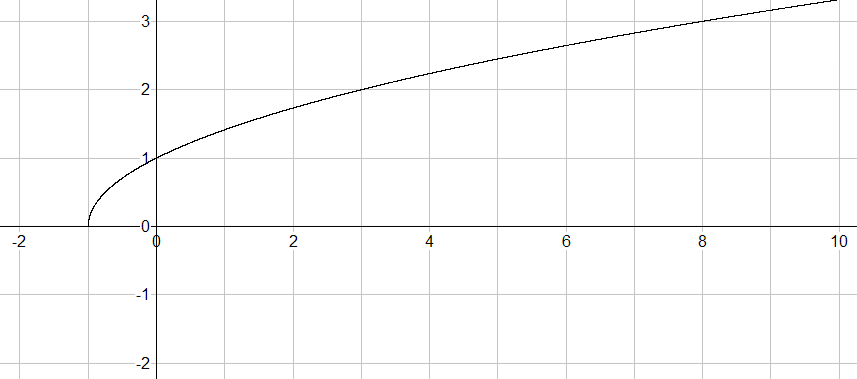
\includegraphics[ width=4.5204in, height=2.0124in,]{L4SZ283J}
}


The curve is clearly continuous. If we let $u =x +1$ then $u^{ \prime } =1$, this is also continuous. 

\textbf{Method 1} 

Substitute $u =x +1$ then $d u =d x$. Substituting these values in the indefinite integral we get
\begin{equation*}\int \sqrt{x +1}\; d x =\int \sqrt{u}\; d u =\frac{2}{3} u^{3/2} +C =\frac{2}{3} \left (x +1\right )^{3/2} +C
\end{equation*}So
\begin{align*}\int _{0}^{8}\sqrt{x +1}\; d x &  = \left .\int \sqrt{x +1}\; d x\right ]_{0}^{8} \\
 &  = \left .\frac{2}{3} \left (x +1\right )^{3/2}\right ]_{0}^{8} \\
 &  = \frac{2}{3} \left (9\right )^{3/2} -\frac{2}{3} \left (1\right )^{3/2} \\
 &  = \frac{2}{3} 27 -\frac{2}{3} 1 \\
 &  = \frac{2}{3} \left (27 -1\right ) =\frac{2}{3} 26 =\frac{52}{3} =17\frac{1}{3}\end{align*}

\textbf{Method 2} 

Again we let $u =x +1$ so $d u =d x$. Also we calculate the new limits for $u$ using $u =x +1$.
\begin{align*}x &  = 0\text{gives}u =0 +1 =1 \\
x &  = 8\text{gives}u =8 +1 =9\end{align*}

Now the definite integral is transformed into a definite integral in $u$. 


\begin{align*}\int _{0}^{8}\sqrt{x +1}\; d x &  = \int _{1}^{9}\sqrt{u}\; d u \\
 &  = \left .\frac{2}{3} u^{3/2}\right ]_{1}^{9} \\
 &  = \frac{2}{3} 9^{3/2} -\frac{2}{3} 1^{3/2} \\
 &  = \frac{2}{3} \left (27 -1\right ) =17\frac{1}{3}\end{align*}

A check on the graph will show that an area of $17\frac{1}{3}$ appears to be reasonable. 

Method 2 is usually preferred as the step where the indefinite integral is first calculated
has been neatly incorporated into the method. The difficulty with method 2 is that once the values for $u$ have been calculated the integral is completely transformed and we never return to the original question. We
answer a different question that, because of the transformation, has the same answer. This concept might cause
confusion. However a graph of the situation shows what has happened. 

   
\setlength\fboxrule{0.01in}\setlength\fboxsep{0.2in}\fcolorbox[HTML]{000000}{FFFFFF}{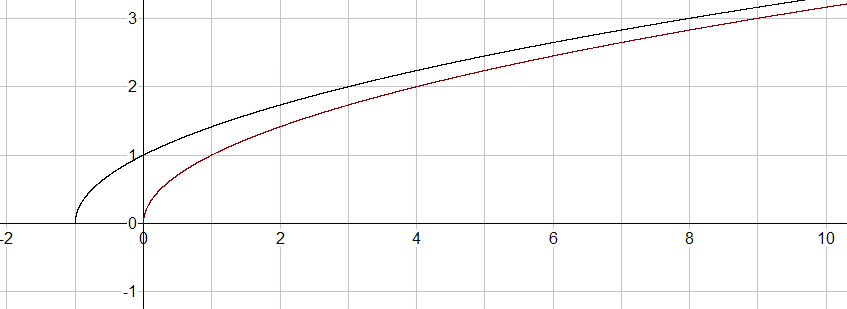
\includegraphics[ width=5.3195in, height=1.9579in,]{L4SZ283K}
}


It is clear that the area under the first graph between $0$ and $8$ is the same as the area under the second graph between $1$ and $9$. 

\subsubsection{Example 2}
Evaluate $\int _{1}^{2}\frac{1}{\left (1 -2 x\right )^{2}}\; d x$ 

A graph shows us the area we are being asked to find. It also shows
that we would not be asked to find an area that includes $x =\frac{1}{2}$. 

   
\setlength\fboxrule{0.01in}\setlength\fboxsep{0.2in}\fcolorbox[HTML]{000000}{FFFFFF}{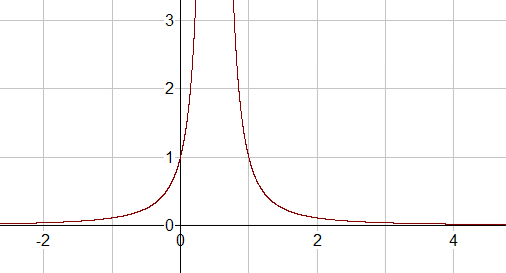
\includegraphics[ width=5.3272in, height=2.8867in,]{L4SZ283L}
}


Let $u =1 -2 x$ so $d u = -2\; d x$ or $d x = -\frac{1}{2}\; d u$. When $x =1$, $u = -1$ and when $x =2$, $u = -3$ 

Using method 2
\begin{align*}\int _{1}^{2}\frac{1}{\left (1 -2 x\right )^{2}}\; d x &  = \int _{ -1}^{ -3}\frac{1}{u^{2}} \cdot \left ( -\frac{1}{2}\right )\; d u \\
 &  =  -\frac{1}{2} \int _{ -1}^{ -3}u^{ -2}\; d u \\
 &  = \left . -\frac{1}{2} \frac{u^{ -1}}{ -1}\right ]_{ -1}^{ -3} \\
 &  = \genfrac{.}{]}{}{}{1}{2 u}_{ -1}^{ -3} \\
 &  = \frac{1}{2 \left ( -3\right )} -\frac{1}{2 \left ( -1\right )} \\
 &  = \frac{1}{ -6} -\frac{1}{ -2} \\
 &  = \frac{1}{2} -\frac{1}{6} =\frac{3 -1}{6} =\frac{2}{6} =\frac{1}{3}\end{align*}

Notice the lower limit for $x$ is transformed into the lower limit for $u$ and the upper limit for $x$ is transformed into the upper limit for $u$. It is important not to get these back to front otherwise the sign will be the opposite
to what it should be. We were expecting the value to be positive because the graph is above the $x$-axis 

\subsection{Exercises 7.5.1}
\begin{enumerate}
\item Evaluate $\int _{0}^{4}\sqrt{2 x +1}\; d x$ 

\item Evaluate $\int _{1}^{2}\frac{1}{\left (3 -5 x\right )^{2}}\; d x$ 

\item Evaluate $\int _{1}^{e}\frac{\ln  x}{x}\; d x$,\qquad $u =\ln  x$ 

\item Evaluate $\int _{0}^{2}\left (x -1\right )^{11}\; d x$ 

\item Evaluate $\int _{0}^{\pi }\sec ^{2} \left (\theta /4\right )\; d \theta $ \end{enumerate}


\subsubsection{Supplementary Exercises}
\begin{enumerate}
\item   
%TCIMACRO{\TeXButton{Start 2 Columns}{\columnsep =30pt
% \begin {multicols}{2}}}%
%BeginExpansion
\columnsep =30pt
\begin {multicols}{2}
%EndExpansion
 $\int _{0}^{2}x \sqrt{2 x^{2} +1}\; d x$ 

\item $\int _{0}^{\frac{\pi }{4}}\sin  \left (x +\frac{\pi }{2}\right )\; d x$ 

\item $\int _{0}^{1}\left (3 -2 x\right )^{4}\; d x$ 

\item $\int _{ -2}^{ -1}\frac{d x}{\left (2 x +1\right )^{2}}$ 

\item $\int _{4}^{9}\frac{d x}{2 x +1}$ 

\item $\int _{0}^{\frac{\pi }{4}}\tan  x\; d x$ 
%TCIMACRO{\TeXButton{End 2 Columns}{\end {multicols}}}%
%BeginExpansion
\end {multicols}
%EndExpansion
  \end{enumerate}


\section{Integration by Parts}
Recall the rule for the differentiation of a product
\begin{equation*}\frac{d}{d x} \left (f (x) \cdot g (x)\right ) =f (x) \cdot g^{ \prime } (x) +g (x) \cdot f^{ \prime } (x)
\end{equation*}

We can antidifferentiate each side and write the process as follows
\begin{align*}f (x) \cdot g (x) &  = \int \left [f (x) \cdot g^{ \prime } (x) +g (x) \cdot f^{ \prime } (x)\right ]\; d x \\
 &  = \int f (x) \cdot g^{ \prime } (x)\; d x +\int g (x) \cdot f^{ \prime } (x)\; d x\end{align*}

This is rewritten in a particular way to become the formula for \emph{integration by parts}.
\begin{align}\int f (x) \cdot g^{ \prime } (x)\; d x &  = f (x) \cdot g (x) -\int g (x) \cdot f^{ \prime } (x)\; d x \tag{1} \\
\text{or}\int f (x) \cdot g^{ \prime } (x)\; d x &  = f (x) \cdot g (x) -\int f^{ \prime } (x) \cdot g (x)\; d x \tag{2}\end{align}

This formula is written in a number of different ways in textbooks. Here
are two ways 

Let $u =f (x)$ and $v =g (x)$ then $d u =f^{ \prime } (x)\; d x$ and $d v =g^{ \prime } (x)\; d x$ so using the substitution rule equation (1) becomes
\begin{equation}\int u\; d v =u v -\int v\; d u\tag{3}
\end{equation}

Let $\int f (x) \cdot g^{ \prime } (x)\; d x$ be regarded as the the integral of the product of two functions then $g =\int g^{ \prime }$. We can write equation (2) as
\begin{equation}\int \left (f \cdot g^{ \prime }\right ) =f \cdot \int  g^{ \prime } -\int \left (f^{ \prime } \cdot \int  g^{ \prime }\right )\tag{4}
\end{equation}

Equation (4) can be said as follows 

The integral of the product of two functions
equals the first function times the integral of the second function minus the integral of the differential of the first function times the integral of the
second function. 

The success of this method depends on the discovery that a simpler integral results from this process. Sometimes
the process results in a worse situation than you started with so should be abandoned. Sometimes you produce
a pattern which leads to a solution after 2 or more applications of the integration by parts rule. The patterns
that produce solvable problems can be discovered as different questions are tried. 

\subsubsection{Example 1}
Find $\int x \cos  x\; d x$ 

This can be seen as the integral of a product. The two functions
are $f (x) =x$ and $g (x) =\cos  x$. So $f^{ \prime } (x) =1$ and $\int g (x) =\sin  x$ are easy to find. Notice though that $f^{ \prime } (x) =1$ gives us a clue that \emph{integration by parts} is going to be a fruitful method. 

Using
equation (2)
\begin{align*}\int x \cos  x\; d x &  = f (x) \cdot g (x) -\int f^{ \prime } (x) \cdot g (x)\; d x \\
 &  = x \cdot \sin  x -\int 1 \cdot \sin  x\; d x \\
 &  = x \cdot \sin  x -\int \sin  x\; d x \\
 &  = x \cdot \sin  x -\left ( -\cos  x\right ) +C \\
 &  = x\; \sin  x +\cos  x +C\end{align*}

Using equation (3). Let $u =x$ and $d v =\cos  x\; d x$. Then $d u =d x$ and $v =\sin  x$. So
\begin{align*}\int x \cos  x\; d x &  = \int u\; d v \\
 &  = u v -\int v\; d u \\
 &  = x\; \sin  x -\int \sin  x\; d x \\
 &  = x\; \sin  x -\left ( -\cos  x\right ) +C \\
 &  = x\; \sin  x +\cos  x +C\end{align*}

\subsubsection{Example 2}
Use integration by parts to find $\int \ln  x\; d x$. This is a function that has arisen in the course as the integral of $\frac{1}{x}$, however we are now able to use this fact to help with this question. notice there is only one function here so we have to create
two functions by stating $\ln  x =1 \cdot \ln  x$. The two functions are therefore $f (x) =\ln  x$ and $g (x) =1$. Can we find $f^{ \prime }$ and $\int g$? Yes!
\begin{align*}\int \ln  x\; d x &  = \int \ln  x \cdot 1\; d x \\
 &  = \ln  x \cdot x -\int \frac{1}{x} \cdot x\; d x \\
 &  = x\; \ln  x -\int 1\; d x \\
 &  = x\; \ln  x -x +C\end{align*}

\subsubsection{Example 3}
Find $\int e^{x} \cos  x\; d x$ 

This is an example where a pattern is established and perseverance leads to the solution. Let
$f (x) =\cos  x$ and $g (x) =e^{x}$. Can we find $f^{ \prime }$ and $\int g$? Yes!
\begin{align*}\int e^{x} \cos  x\; d x &  = \cos  x \cdot e^{x} -\int  -\sin  x \cdot e^{x}\; d x \\
 &  = e^{x} \cos  x +\int e^{x} \sin  x\; d x\end{align*}

This is an integral that is very similar in appearance to the original question with the $\cos  x$ transformed into $\sin  x$. We continue by repeating the integration by parts process with the new integral
$\int e^{x} \sin  x\; d x$
\begin{align*}\int e^{x} \cos  x\; d x &  = e^{x} \cos  x +\overset{\int e^{x} \sin  x\; d x}{\overbrace{\sin  x \cdot e^{x} -\int \cos  x \cdot e^{x} d x}} \\
 &  = e^{x} \cos  x +e^{x} \sin  x -\int e^{x} \cos  x\; d x\end{align*}

Notice the original integral has now appeared on the right hand side of the equation. We
now simply solve the equation for $\int e^{x} \cos  x\; d x$ and add the constant of integration.
\begin{align*}2 \int e^{x} \cos  x\; d x &  = e^{x} \cos  x +e^{x} \sin  x \\
\int e^{x} \cos  x\; d x &  = \frac{e^{x}}{2} \left (\cos  x +\sin  x\right ) +C\end{align*}

This can easily be verified as correct by differentiating. 

\subsection{Exercises 7.6.1}
\begin{enumerate}
\item Find $\int x \ln  x\; d x$ 

\item Find $\int x \sin  x\; d x$ 

\item Find $\int x \cos  3 x\; d x$ 

\item Find $\int e^{x} \sin  x\; d x$ 

\item Find $\int \ln  \left (2 x\right )\; d x$ 

\item By writing $\sin ^{2} x$ as $\sin  x \cdot \sin  x$ and using integration by parts show
\begin{equation*}\int \sin ^{2} x\; d x =\frac{1}{2} \left (x -\sin  x \cdot \cos  x\right ) +C
\end{equation*}\end{enumerate}


\subsubsection{Supplementary Exercises}
\begin{enumerate}
\item $\int x e^{2 x}\; d x$ 

\item $\int x e^{ -x}\; d x$ 

\item $\int x^{2} \sin  x\; d x$ 

\item $\int \left (x -1\right ) e^{x}\; d x$ 

\item $\int \frac{\ln  x}{x}\; d x$ \end{enumerate}


\subsection{Definite Integrals}
Integration by parts can be combined with the Evaluation Theorem to evaluate definite integrals. If
we assume $f^{ \prime }$ and $g^{ \prime }$ are continuous then we can use the Evaluation Theorem and write equation (1) as follows
\begin{equation}\int _{a}^{b}f (x) \cdot g^{ \prime } (x)\; d x =\left .f (x) \cdot g (x)\right ]_{a}^{b} -\int _{a}^{b}g (x) \cdot f^{ \prime } (x)\; d x\tag{5}
\end{equation}

\subsubsection{Example 4}
Evaluate $\int _{0}^{1}x e^{x}\; d x$ 

A graph of $y =x e^{x}$ shows the area required and gives us an idea of the answer to expect. 

   
\setlength\fboxrule{0.01in}\setlength\fboxsep{0.2in}\fcolorbox[HTML]{000000}{FFFFFF}{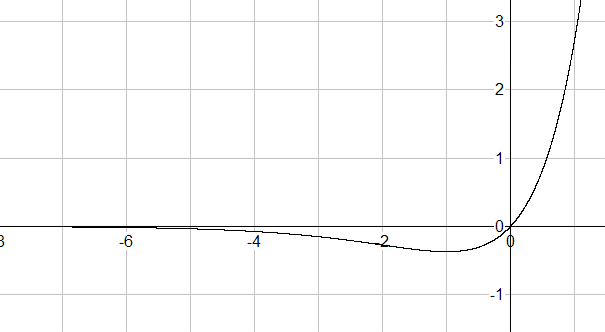
\includegraphics[ width=4.7374in, height=2.6126in,]{L4SZ283M}
}


Notice $x$ becomes simpler when differentiated and $e^{x}$ is unchanged when it is integrated
\begin{align*}\int _{0}^{1}x e^{x}\; d x &  = \left .x e^{x}\right ]_{0}^{1} -\int _{0}^{1}1 \cdot e^{x}\; d x \\
 &  = \left .x e^{x}\right ]_{0}^{1} -\left .e^{x}\right ]_{0}^{1} \\
 &  = \left (\left (1 e^{1}\right ) -\left (0 e^{0}\right )\right ) -\left (e^{1} -e^{0}\right ) \\
 &  = e^{1} -e^{1} +e^{0} \\
 &  = e^{0} =1\end{align*}

\subsection{Exercises 7.6.2}
\begin{enumerate}
\item Evaluate $\int _{0}^{5}x e^{ -x}\; d x$ 

\item Evaluate $\int _{0}^{1}x^{2} e^{x}\; d x$ 

\item Evaluate $\int _{0}^{\pi }e^{x} \sin  x\; d x$ 

\item $\int _{1}^{3}x \ln  x\; d x$ 

\item $\int _{0}^{\pi }\sin ^{2} x\; d x$ \end{enumerate}


\subsubsection{Supplementary Exercises}
\begin{enumerate}
\item $\int _{0}^{\frac{\pi }{2}}x \sin  x\; d x$ 

\item $\int _{0}^{1}x e^{2 x}\; d x$ 

\item $\int _{5}^{7}x \cos  x\; d x$ 

\item $\int _{1}^{2}\left (x -1\right ) e^{x}\; d x$ 

\item $\int _{2}^{4}\frac{\ln  x}{x}\; d x$ 

\item $\int _{0}^{3}x^{2} \sin  x\; d x$ \end{enumerate}


 

\section{Applications of Integration}


\subsection{Rectilinear Motion}
We will use integration to analyse the motion of an object moving in a straight line. Let
the position function for the object be $s =f (t)$ where $t$ is the time. The velocity function is $v (t) =s^{ \prime } (t)$. Therefore the position function is the integral of the velocity function. Also
the acceleration function is $a (t) =v^{ \prime } (t)$ so the velocity function is the integral of the acceleration function. We can obtain
the position function from the acceleration function by antidifferentiating twice. This process will generate
two constants of integration so we need two additional pieces of information to find the particular solution. Usually
$s (0)$ and $v (0)$ are given. 

\subsubsection{Example 1}
A particle moves in a straight line with an acceleration of $a (t) =4 t +2$. If the initial velocity is $ -4 \mbox{cm}$/$\mbox{s}$ and the initial displacement is $5 \mbox{cm}$, find the position function. 

Because $v^{ \prime } (t) =a (t) =4 t +2$ we can antidifferentiate $a (t)$ to obtain $v (t)$
\begin{equation*}v (t) =4 \frac{t^{2}}{2} +2 t +C_{1} =2 t^{2} +2 t +C_{1}
\end{equation*}

Substitute $t =0$ because we are given the initial velocity i.e. $v (0) = -4$
\begin{align*}v (0) &  = 2 \cdot 0^{2} +2 \cdot 0 +C_{1} = -4 \\
\text{So}C_{1} &  =  -4\text{and therefore} \\
v (t) &  = 2 t^{2} +2 t -4\end{align*}

Because $s^{ \prime } (t) =v (t)$ we can antidifferentiate $v (t)$ to obtain $s (t)$.
\begin{align*}s (t) &  = 2 \frac{t^{3}}{3} +2 \frac{t^{2}}{2} -4 t +C_{2} \\
 &  = \frac{2}{3} t^{3} +t^{2} -4 t +C_{2}\end{align*}

Substitute $t =0$ because we are given the initial displacement i.e. $s (0) =5$
\begin{align*}s (0) &  = \frac{2}{3} \cdot 0^{3} +0^{2} -4 \cdot 0 +C_{2} =5 \\
\text{So}C_{2} &  = 5\text{and therefore} \\
s (t) &  = \frac{2}{3} t^{3} +t^{2} -4 t +5\end{align*}

You should know about the gravitational force near the earth that produces a downwards acceleration
given the symbol $g$. We assume $g$ is constant and about $9.8 \mbox{m}$/$\mathrm{s}^{2}$ 

\subsubsection{Example 2}
A ball is thrown vertically upwards with a speed of $24.5 \mbox{m}$/$\mbox{s}$ from the edge of a cliff that is $147 \mbox{m}$ above the ground. 


\begin{description}
\item [(a)] Find the position function. 

\item [(b)]
Find the time when the ball reaches its maximum height 

\item [(c)]
Find the maximum height above the ground 

\item [(d)] When
does the ball hit the ground? \end{description}

(a) It is usual to choose the positive direction
to be upwards this means that the acceleration due to gravity must be $ -9.8 \mbox{m}$/$\mathrm{s}^{2}$.
\begin{align*}\text{So}a (t) &  = v^{ \prime } (t) = -9.8\text{therefore} \\
v (t) &  =  -9.8 t +C_{1}\end{align*}

Substituting $v (0) =24.5$ we get that $C_{1} =24.5$ so
\begin{equation*}v (t) = -9.8 t +24.5
\end{equation*}

Because $s^{ \prime } (t) =v (t)$ we antidifferentiate $v (t)$
\begin{equation*}s (t) = -9.8 \frac{t^{2}}{2} +24.5 t +C_{2}
\end{equation*}

Substitute $s (0) =147$. We get $C_{2} =147$.
\begin{equation*}\text{So}s (t) = -4.9 t^{2} +24.5 t +147
\end{equation*}

This expression will hold true until the ball hits the ground provided you assume the ball continues
on its trajectory without striking the cliff. 

(b) The maximum height is reached when $v (t) =0$.
\begin{align*} -9.8 t +24.5 &  = 0 \\
24.5 &  = 9.8 t \\
t &  = \frac{24.5}{9.8} \\
 &  = 2.5\end{align*}

So the maximum height is reached after $2.5 \mbox{s}$. 

(c) The maximum height is found by substituting
$t =2.5$ in $s (t)$
\begin{align*}s (2.5) &  =  -4.9 \cdot 2.5^{2} +24.5 \cdot 2.5 +147 \\
 &  =  -30.625 +61.25 +147 =177.625 \mbox{m}\end{align*}

(d) The ball hits the ground when $s (t) =0$
\begin{align*}\text{So} -4.9 t^{2} +24.5 t +147 &  = 0 \\
t^{2} -5 t -30 &  = 0\end{align*}

Use the quadratic formula $t =\frac{ -b \pm \sqrt{b^{2} -4 a c}}{2 a}$
\begin{align*}t &  = \frac{5 \pm \sqrt{25 -4 \times 1 \times  -30}}{2} \\
 &  = \frac{5 \pm \sqrt{145}}{2} \\
 &  \approx 8.5\text{}\mbox{s}\text{or} -3.5\text{}\mbox{s}\end{align*}

You will be aware that the position function is a parabola so it is not surprising that the theoretical
result shows a solution about $3.5 \mbox{s}$ before the ball is thrown. The
answer is that the ball hits the ground about $8.5 \mbox{s}$ after it is thrown. You will
also be aware that we did not test whether the value of $t$ when $v (t) =0$ gives a maximum or minimum. This is also because we are aware of the behaviour of
a parabola with a negative $t^{2}$ coefficient. 

\subsection{Exercises 7.7.1}
\begin{enumerate}
\item A particle is moving in a straight line with an acceleration given by $a (t) =6 t +4.$ Its initial velocity is $v (0) = -6 cm/\mbox{s}$ and its initial displacement is $s (0) =9 \mbox{cm}$. Find the position function $s (t)\text{.}$ 

\item A ball is thrown upwards with an initial velocity of $15 \mathrm{m}/\mbox{s}$ from the edge of a cliff $140 \mbox{m}$ above the ground. Find its
height above the ground $t$ seconds later. When does it reach its maximum height? When
does it hit the ground? 

\item A particle is moving along a straight line with an acceleration of $a (t) =3 +4 t -12 t^{2}$. Its initial velocity, $v (0)$ is $4 \mbox{m}$/$\mbox{s}$ and its initial displacement, $s (0)$ is $5 \mbox{m}$. Find the position function,
$s (t)$. 

\item A stone is dropped off a cliff and hits the ground with a speed of $40 \mbox{m}$/$\mbox{s}$. What is the height of the
cliff? 

\item A car is travelling at $50 \mbox{km}$/$\mbox{h}$ when the brakes are firmly applied producing a constant deceleration of
$5$ $\mbox{m}$/$\mathrm{s}^{2}$. How far will the car travel before coming to rest? 

\item A
car is travelling at $100 \mbox{km}$/$\mbox{h}$ when the driver sees a railway crossing $80 \mbox{m}$ ahead and "slams on the brakes". What
constant deceleration is required so that the car will stop in $80 \mbox{m}$? 

\item Two balls are
thrown upwards from the edge of the cliff in exercise 2 above. The first is thrown with a speed of $15 \mathrm{m}/\mbox{s}$ and the second is thrown one second later with a speed of $8 \mathrm{m}/\mbox{s}$. Do the balls ever pass each other? 

\item A
particle moves along a straight line with a velocity function $v (t) =\sin  t -\cos  t$ and its initial displacement is $s (0) =0 \mbox{m}$. Find its position function 

\item A
car braked with a constant deceleration $5 \mathrm{m}/\mathrm{s}^{2}$, producing skid marks measuring $60 \mbox{m}$ before coming to rest. How
fast was the car travelling when the brakes were first applied? \end{enumerate}


\subsection{Work}
The strategy we use to allow us to apply calculus to a problem in engineering is the same as we used to evaluate areas. The
physical quantity is divided up into a large number of small parts, each one approximately equal to the theoretical quantity it represents. These
are then summed and a limit taken as the number of small parts, $n \rightarrow \infty $. This process allows us to evaluate the resulting integral. 

You
will recall that from Newton's Second Law of Motion
\begin{equation}F =m a =m \frac{d^{2} s}{d t^{2}}\tag{1}
\end{equation}

Where $s (t)$ is the position function, $m$ is the mass of an object and $F$ is the force required to produce an acceleration of $a$. (Where $a =\frac{d^{2} s}{d t^{2}}$). 

We usually measure mass in kilograms ($\mbox{kg}$), distance in metres ($\mbox{m}$) and force in Newtons ($\mbox{N}$) \linebreak\relax ($N =k g \cdot m/s^{2}$). If the acceleration is constant then the force to produce that acceleration will also
be constant. 

Work = force $ \times $ distance or
\begin{equation}W =F d\tag{2}
\end{equation}If $F$ is in Newtons and $d$ is in metres then $W$ is in Newton-metres. One Newton-metre is called a\linebreak\relax Joule
($\mbox{J}$). 

\subsubsection{Example 1}
A mass of $3.5 \mbox{kg}$ lifted $0.5 \mbox{m}$ requires a force of
\begin{equation*}F =m a =3.5 \times 9.8 =34.3 \mbox{N}
\end{equation*}

This is the force required to counter the force exerted by gravity. 

The work
done is calculated using equation 2
\begin{equation*}W =F d =34.3 \times 0.5 =17.15 \mbox{J}
\end{equation*}

If the force is variable this formula can no longer be applied. Let
the force acting on an object as it moves along the $x$-axis in a positive direction from $a$ to $b$ be $f (x)$, where $f$ is a continuous function of $x$. Divide the interval from $a$ to $b$ into $n$ subintervals of width $ \Delta x$ where $ \Delta x =\frac{b -a}{n}$. For
simplicity we let the end points of these subintervals be $x_{0}$, $x_{1}$, $x_{2}$, ..., $x_{n}$ We select the $i^{t h}$ subinterval and select a representative $x$-value in this interval $x_{i}^{ \ast }$. The work done when we move the object from $x_{i -1}$ to $x_{i}$ is
\begin{equation*}W_{i} \approx f (x_{i}^{ \ast })  \Delta x
\end{equation*}

The total work done is
\begin{equation}W =\sum _{i =1}^{n}f (x_{i}^{ \ast })  \Delta x\tag{3}
\end{equation}

As we did with area we find the limit as $n \rightarrow \infty $ of this sum. As this is a Riemann sum the limit is a definite integral
\begin{equation}W =\sum _{i =1}^{n}f (x_{i}^{ \ast })  \Delta x =\int _{a}^{b}f (x)\; d x\tag{4}
\end{equation}

\subsubsection{Example 2}
If the force on a particle is given by the equation $f (x) =3 x^{2} -2 x \mbox{N}$, how much work is done moving the particle from $x =2$ to $x =3$. 

The graph of $f (x) =3 x^{2} -2 x$ shows that for the interval $\left [2 ,3\right ]$ the area is above the $x$-axis.
\begin{align*}W &  = \int _{a}^{b}f (x)\; d x \\
 &  = \int _{2}^{3}\left (3 x^{2} -2 x\right )\; d x \\
 &  = \left .3 \frac{x^{3}}{3} -2 \frac{x^{2}}{2}\right ]_{2}^{3} \\
 &  = \left .x^{3} -x^{2}\right ]_{2}^{3} \\
 &  = \left (3^{3} -3^{2}\right ) -\left (2^{3} -2^{2}\right ) \\
 &  = 18 -4 =14\end{align*}

Work done is $14 \mbox{J}$ 

\subsubsection{Example 3}
Hooke's Law states that the force required to maintain a spring stretched $x$ units beyond its natural length is proportional to $x$.
\begin{equation*}f (x) =k x
\end{equation*}

where $k$ is the spring constant. This law holds provided $x$ does not get too large. A force of $20 \mbox{N}$ is required to stretch a spring from its natural length of $5 \mbox{cm}$ to a length of $7 \mbox{cm}$. How much work is required to stretch the spring
from a length of $12 \mbox{cm}$ to $13 \mbox{cm}$? 

As the force is measured in Newtons we convert all lengths to metres.
\ Our first step is to use Hooke's Law to evaluate the spring constant
\begin{align*}f (x) &  = k x \\
\text{So}20 &  = k \cdot 0.02 \\
k &  = 1000 \\
\text{So}f (x) &  = 1000 x\end{align*}

The work done in stretching the spring from $12 \mbox{cm}$ to $13 \mbox{cm}$ is
\begin{align*}W &  = \int _{0.07}^{0.08}1000 x\; d x \\
 &  = \left .500 x^{2}\right ]_{0.07}^{0.08} \\
 &  = 500 \left (0.08^{2} -0.07^{2}\right ) \\
 &  = 500 \left (0.0064 -0.0049\right ) =500 \times 0.0015 \\
 &  = 0.75\text{}\mbox{J}\end{align*}

\subsection{Exercises 7.7.2}
\begin{enumerate}
\item A particle is moved along the $x$-axis by a force given by the equation $f (x) =6/\left (1 +x\right )^{2} \mbox{N}$ at a point $x$ metres from the origin. Find the work done in moving the particle from the origin
to a distance of $5$ metres. 

\item When a particle is located a distance of $x$ metres from the origin a force of $\cos  \left (\pi  x/3\right )$ Newtons acts on it. How much work is done in moving the particle from $x =1$ to $x =2$? Interpret your answer by considering the work done from $x =1$ to $x =1.5$ and from $x =1.5$ to $x =2$. By drawing the graph of $y =\cos  \left (\pi  x/3\right )$ the reason should become apparent. 

\item \  \\\relax
%TCIMACRO{\TeXButton{Start 2 Columns}{\columnsep =30pt
% \begin {multicols}{2}}}%
%BeginExpansion
\columnsep =30pt
\begin {multicols}{2}
%EndExpansion
    
\setlength\fboxrule{0in}\setlength\fboxsep{0.2in}\fcolorbox[HTML]{000000}{FFFFFF}{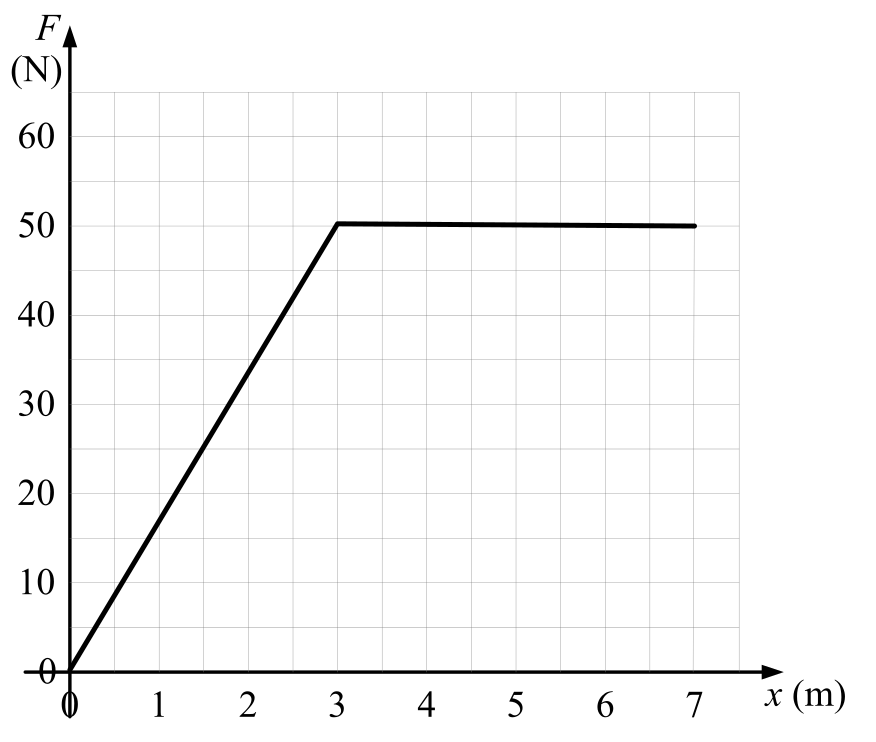
\includegraphics[ width=2.3748in, height=2.015in,]{L4SZ283N}
}
\\\relax The graph shows a force function . (Force in Newtons
against distance in metres.) The force increases at a constant rate until it reaches its maximum value then
remains constant. How much work is done by the force in moving an object a distance of $7 \mbox{m}$? 
%TCIMACRO{\TeXButton{End 2 Columns}{\end {multicols}}}%
%BeginExpansion
\end {multicols}
%EndExpansion


\item A spring has a natural length of $20 \mbox{cm}$. If a $25 \mbox{N}$ force is required to keep it stretched to a length of $30$ $\mbox{cm}$ how much work is done stretching it from a length of $20 \mbox{cm}$ to $25 \mbox{cm}$? 

\item Suppose that $2 \mbox{J}$ of work is needed to stretch a spring from its natural length of $20 \mbox{cm}$ to a length of $30 \mbox{cm}$. How much work is needed to stretch it from a length
of $22 \mbox{cm}$ to $28 \mbox{cm}$? 

\item If $6 \mbox{J}$ of work is needed to stretch a spring from $10 \mbox{cm}$ to $12 \mbox{cm}$ and $10 \mbox{J}$ is needed to stretch it from $12 \mbox{cm}$ to $14 \mbox{cm}$, what is the natural length of the spring? \end{enumerate}


\section{Numerical Integration}
When we introduce the subject of integration we do so with a range of functions that we know will have an integral. In
fact many situations arise in practice where the integral is difficult or impossible to find and of course if we cannot find the integral we
cannot use the Evaluation Theorem. In other situations we may have a table of values we have obtained from an
experiment and the process of fitting a curve to the data may prove unsatisfactory. 

In these cases we use an approximate method to
evaluate a definite integral. There are a number of approximate methods. The
left sum and right sum we met earlier are examples. Another very similar method uses the mid-point of every
interval. A fourth method that is quite popular is called the trapezoidal method which creates a trapezium out
of each subinterval and finds the area of the sum of the $n$ trapeziums. 

\bigskip We usually set up a spreadsheet to evaluate the sum as
the process is to select a sufficiently large value of $n$ so that the rectangles or trapeziums approximate the curve. Very large values of
$n$ will result in the round-off errors accumulating to make the result less reliable so a compromise must be reached where the
value of $n$ is large enough without being too large. 

\subsection{Simpson's Rule}
Another rule to find the approximate integral is Simpson's Rule. This uses parabolas to approximate the curve rather than straight lines as for
the previous $4$ rules. The process is the same for each method. We
select a value for $n$ then tabulate the values of $f (x)$\ for the $n +1$ values of $x_{i}$. In this course we will only cover Simpson's Rule and use it as an example of the 5 methods
available. 

A unique parabola can be drawn through $3$ consecutive points. $n$ must be an even number for us to be able to use Simpson's Rule. For example let
$n =6$. To find the area under the curve $y =f (x)$ between $x =a$ and $x =b$ the first step is to make 6 strips and to tabulate the results. 

\qquad \qquad \qquad \qquad \qquad
\begin{tabular}[c]{|c|c|c|c|c|c|c|}\hline
$x_{0}$  & $x_{1}$  & $x_{2}$  & $x_{3}$  & $x_{4}$  & $x_{5}$  & $x_{6}$  \\
\hline
$f (x_{0})$  & $f (x_{1})$  & $f (x_{2})$  & $f (x_{3})$  & $f (x_{4})$  & $f (x_{5})$  & $f (x_{6})$  \\
\hline
\end{tabular}

A unique parabola can be drawn through $f (x_{0})$, $f (x_{1})$ and $f (x_{2})$ and through $f (x_{2})$, $f (x_{3})$ and $f (x_{4})$ and finally through $f (x_{4})$, $f (x_{5})$ and $f (x_{6})$.\ The pattern is assured because $n$ is even. 

Simpson's Rule can be proved and the proof can be found in calculus textbooks. We
will not prove the rule in this course but will instead concentrate on the way it is used. The formula will
be given on the formula sheet should you require it. 

The formula is
\begin{equation}\int _{a}^{b}f (x)\; d x \approx \frac{ \Delta x}{3} \left (\begin{array}{c}f (x_{0}) +4 f (x_{1}) +2 f (x_{2}) +4 f (x_{3}) +\ldots  \\
 +2 f (x_{n -2}) +4 f (x_{n -1}) +f (x_{n})\end{array}\right )\tag{1}
\end{equation}

Where $n$ is even and $ \Delta x =\left (b -a\right )/n$. 

It is usual to number the subscripts in this way so that the pattern can help with the setting out of a solution.
\ Notice $f (x_{0})$ and $f (x_{n})$ have coefficients of 1; $f (x_{1})$, $f (x_{3})$ etc. have coefficients of $4$ and these are the ones with a subscript that is an odd number; and $f (x_{2})$, $f (x_{4})$ etc. have coefficients of $2$ and these are the ones with a subscript that is an even number. So Simpson's Rule is sometimes written as follows
\begin{equation}\int _{a}^{b}f (x)\; d x \approx \frac{ \Delta x}{3} \left (f (x_{0}) +f (x_{n}) +4 \left (f (x_{1}) +f (x_{3}) +\ldots \right ) +2 \left (f (x_{2}) +f (x_{4}) +\ldots \right )\right )\tag{2}
\end{equation}

\subsubsection{Example}
It is usual to practice Simpson's Rule with an exercise that you do in fact know the answer to so that the accuracy of the method can be explored.
\ Use Simpson's Rule to evaluate $\int _{1}^{2}\frac{1}{x}\; d x$ with $n =10$. 

Firstly $\int _{1}^{2}\frac{1}{x}\; d x =\left .\ln  x\right ]_{1}^{2} =\ln  2 -\ln  1 =0.69314718$ so we can verify the accuracy of any answer we get. 

Using Simpson's rule $ \Delta x =(2 -1)/10 =0.1$ so 


\begin{align*}\int _{1}^{2}\frac{1}{x}\; d x &  \approx \frac{0.1}{3} \left (\frac{1}{1} +\frac{1}{2} +4 (\frac{1}{1.1} +\frac{1}{1.3} +\frac{1}{1.5} +\frac{1}{1.7} +\frac{1}{1.9}) +2 \left (\frac{1}{1.2} +\frac{1}{1.4} +\frac{1}{1.6} +\frac{1}{1.8}\right )\right ) \\
 &  = \frac{0.1}{3} \left (1.5 +13.83815771 +5.456349206\right ) =\frac{0.1}{3} \left (20.79450692\right ) =0.69315023\end{align*}

It is immediately clear that this is a very good approximation. 

\subsection{Exercises 7.8.1}
\begin{enumerate}
\item Use Simpson's Rule with the value of $n$ given to find the area in each case 


\begin{description}
\item [(a)] $\int _{0}^{2}e^{x}\; d x$, $n =10$. Verify the result by integration. 

\item [(b)]
$\int _{0}^{2}\sqrt{4 -x^{2}}\; d x$, $n =8$. Verify the result by noting that $y =\sqrt{4 -x^{2}}$ is a semicircle so the required area can be found by formula. 

\item [(c)]
$\int _{0}^{2}e^{ -x^{2}}\; d x$, $n =10$. Draw the graph of $y =e^{ -x^{2}}$ to show the area being calculated. This is an example of a function that cannot be integrated
so an approximate integral has to be found should we be asked to find this area. \end{description}

\item The
following table gives the results of an experiment \end{enumerate}


\qquad \qquad \qquad \qquad \qquad
\begin{tabular}[c]{|c|c|c|c|c|c|c|c|c|}\hline
$0$  & $0.5$  & $1$  & $1.5$  & $2$  & $2.5$  & $3$  & $3.5$  & $4$  \\
\hline
$0$  & $1$  & $3$  & $4.5$  & $5$  & $4.5$  & $3$  & $2$  & $1$  \\
\hline
\end{tabular}


\begin{enumerate}
\item [] Use Simpson's Rule to find the area under the graph drawn from these data.


\item [3.] A radar gun was used to record the speed of a runner during
the first 5 seconds of a race. The data are collected in the table below. Use
Simpson's Rule to estimate the distance the runner covered during those 5 seconds. \end{enumerate}


\qquad \qquad \qquad \qquad \qquad \qquad
\begin{tabular}[c]{|c|c||c|c|}\hline
$t$ ($\mbox{s}$)  & $v$ ($\mbox{m}$/$\mbox{s}$)  & $t$ ($\mbox{s}$)  & $v (\mathrm{m}/\mbox{s})$  \\
\hline
$0$  & $0$  & $3.0$  & $10.51$  \\
$0.5$  & $4.67$  & $3.5$  & $10.67$  \\
$1.0$  & $7.34$  & $4.0$  & $10.76$  \\
$1.5$  & $8.86$  & $4.5$  & $10.81$  \\
$2.0$  & $9.73$  & $5.0$  & $10.81$  \\
$2.5$  & $10.22$  &  &  \\
\hline
\end{tabular}


\begin{enumerate}
\item [4.] The table shows a force function $f (x)$ where $x$ is measured in metres and $f (x)$ in Newtons. Use Simpson's Rule to estimate the work done by the force in moving an object
a distance of $18 \mbox{m}$. \end{enumerate}


\qquad \qquad \qquad \qquad \qquad \qquad \qquad
\begin{tabular}[c]{|c|c|c|c|c|c|c|c|}\hline
$x$  & $0$  & $3$  & $6$  & $9$  & $12$  & $15$  & $18$  \\
\hline
\hline
$f (x)$  & $9.8$  & $9.1$  & $8.5$  & $8.0$  & $7.7$  & $7.5$  & $7.4$  \\
\hline
\end{tabular}

 

\section{Answers}
%TCIMACRO{\TeXButton{Start Two Columns}{\columnsep =30pt
% \begin {multicols}{2}}}%
%BeginExpansion
\columnsep =30pt
\begin {multicols}{2}
%EndExpansion
 

\textbf{Exercise 7.1.1} 

1(a) $\;3 x +C\text{\quad \quad }$(b) $x^{3} -\frac{x^{4}}{2} +C$ 

1(c) $\frac{3 x^{5/3}}{5} -\frac{15 x^{2/3}}{2} +C\text{\quad \quad }$(d) $\sqrt{x} +\frac{x}{\sqrt{2}} +C$ 

2(a) $\frac{5 x^{3}}{3} +C\text{\quad \quad }$(b) $x -\ln  \left \vert x\right \vert  +C$ 

3. $3 x^{2} +C x +D$ 

Supplementary Exercises 

1. $\;\frac{x^{8}}{2} +C\text{\quad \quad }$2. $10 x +C$ 

3. $\frac{2}{3} x^{4} +C\text{\quad \quad }$4. $3.2 e^{x}$ 

5. $\frac{1}{2} \ln  \left \vert x\right \vert  +C\text{\quad \quad }$6. $\frac{2 x^{3/2}}{3} +C$ 

7. $\frac{x^{2.2}}{2.2} +C\text{\quad \quad }$8. $\;\frac{x^{\pi  +1}}{\pi  +1} +C$ 

9. $\frac{ -12}{\sqrt[{3}]{x}} +C\text{\quad \quad }$10. $3 \sqrt[{3}]{x} +C$ 

11. $\frac{4}{3} x^{3} +2 x^{2} +x +C\text{\quad \quad }$12. $e^{x} +\frac{x^{e +1}}{e +1} +C$ 

\textbf{Exercises 7.2} 

1. $\frac{\pi }{4}\text{\quad \quad }$2. $12$ 

3. $7.5\text{\quad \quad }$4. $2.5$ 

\textbf{Exercises 7.3.1} 

1(a) $\frac{21}{2}\text{\quad \quad }$(b) $ -70$ 

1(c) $\frac{3}{5}\text{\quad \quad }$(d) $e^{3} -e$ 

1(e) $\ln  3$ 

2(a) $20\frac{1}{2}\text{\quad \quad }$(b) $9\frac{1}{3}$ 

Supplementary Exercises 

1. $\frac{2}{3}\text{\quad \quad }$2. $ -1\frac{1}{2}$ 

3. $\frac{1}{3} \ln  \frac{3}{2} \approx 0.135$ (3dp) 

4. $3 \left (e -1\right ) \approx 5.155$ (3dp) 

5. $12\frac{4}{5}$ 

6. $\frac{1}{4} -\frac{1}{4} =0$ Area $ =\frac{1}{2}$ 

\textbf{Exercises 7.4} 

1. $\frac{x^{2}}{2} +x^{ -1} +C$ 

2. $\frac{2 \sqrt{x^{5}}}{5} +C$ 

3. $ -\cos  x -2 \sin  x +C$ 

4. $2 x -\frac{3}{2} x^{2} +\frac{x^{3}}{3} +C$ 

5. $x +C$ 

6. $2 \ln  \left \vert x\right \vert  +6 \sqrt{x} +C$ 

Supplementary Exercises 

1. $\frac{1}{2} \sin  x +C$ 

2. $\frac{1}{2} \tan  x +C$ 

3. $\frac{x^{2}}{2} +x +\ln  \left \vert x\right \vert  +C$ 

4. $\pi  r^{2} x +\frac{\pi  x^{3}}{3} +C$ 

5. $\frac{1}{2} \ln  \left \vert x\right \vert  +C$ 

6. $\pi  r^{2} +C$ 

\textbf{Exercises 7.5} 

1. $\;\frac{1}{4} e^{4 x} +C$ 

2. $\ln  \left \vert \cos  x\right \vert  +C$ 

3. $e^{\sin  \theta } +C$ 

4. $\frac{1}{64} \left (4 x -3\right )^{16} +C$ 

5. $\frac{1}{2} e^{x^{2}} +C$ 

6. $\frac{1}{2} \ln  \left (x^{2} +1\right ) +C$ as $x^{2} +1$ is always positive 

Supplementary Exercises 

1. $\;\frac{1}{4} \left (x^{2} +2\right )^{4} +C$ 

2. $\frac{1}{3} \sin ^{3} x +C$ 

3. $\frac{2 \sqrt{\left (1 +x\right )^{3}}}{3} -2 \sqrt{1 +x} +C$ 

4. $2 \ln  \left (1 +\sqrt{x}\right ) +C$ as $1 +\sqrt{x}$ is always positive 

5. $\frac{1}{3} \left (2 x +1\right )^{3/2} +C$ 

6. $2 \sqrt{x +1} +C$ 

7. $\ln  \left (e^{x} +1\right ) +C$ as $e^{x} +1$ is always positive 

8. $\frac{1}{2} \left (\ln  x\right )^{2} +C ,x >0$ because $\frac{\ln  x}{x}$ does not exist when $x \leq 0$ 

9. $\frac{2}{3} \sqrt{\sin ^{3} x} +C$ 

10. $\ln  \left \vert \sin  x +1\right \vert  +C$ 

11. $2 \sin  \frac{x}{2} +C\text{\quad \quad }$12. $\frac{1}{2} \sin  2 x +C$ 

13. $\frac{e^{x} -e^{ -x}}{2} +C\text{\quad \quad }$14. $ -e^{1 -x} +C$ 

\textbf{Exercises 7.5.1} 

1. $\frac{26}{3}\text{\quad \quad }$2. $\frac{1}{14}$ 

3. $\;\frac{1}{2}\text{\quad \quad }$4. $0\text{,}$ Area $ =\frac{1}{12} \times 2 =\frac{1}{6}$ 

5. $4$ 

Supplementary Exercises 

1. $4\frac{1}{3}\text{\quad \quad }$2. $\frac{\sqrt{2}}{2}$ 

3. $\frac{121}{5} =24.2\text{\quad \quad }$4. $ -\frac{5}{12}$ 

5. $\frac{1}{2} \ln  \frac{19}{9} \approx 0.374$ (3dp) 

6. $\ln  \frac{\sqrt{2}}{2} = -0.347\text{,}$ Area $ =0.347$ (3dp) 

\textbf{Exercises 7.6.1} 

1. $\;\frac{x^{2}}{2} \ln  x -\frac{x^{2}}{4} +C$ 

2. $\sin  x -x \cos  x +C$ 

3. $\frac{x}{3} \sin  3 x +\frac{1}{9} \cos  3 x +C$ 

4. $\;\frac{1}{2} e^{x} \left (\sin  x -\cos  x\right ) +C$ 

5. xln$\left \vert 2 x\right \vert  -x +C$ 

Supplementary Exercises 

1. $\frac{1}{2} x e^{2 x} -\frac{1}{4} e^{2 x} +C$ 

2. $ -e^{ -x} \left (x +1\right ) +C$ 

3. $ -x^{2} \cos  x +2 x \sin  x +2 \cos  x +C$ 

4. $e^{x} \left (x -2\right ) +C$ 

5. $\frac{1}{2} \left (\ln  x\right )^{2} +C ,x >0$ because $\frac{\ln  x}{x}$ does not exist when $x \leq 0$ 

\textbf{Exercises 7.6.2} 

1. $ -6 e^{ -5} +1 \approx 0.9596$ (4 dp) 

2. $e -2 \approx 0.718$ 

3. $\frac{1}{2} \left (e^{\pi } +1\right ) \approx 12.07$ 

4. $\frac{9}{2} \ln  3 -\frac{1}{2} \ln  1 -2 \approx 2.9$ 

5. $\frac{\pi }{2} \approx 1.57$ 

Supplementary Exercises 

1. $\;1$ 

2. $\frac{1}{4} \left (e^{2} -1\right ) \approx 1.597$ (3dp) 

3. $\;7 \sin  7 +\cos  7 -\left (5 \sin  5 +\cos  5\right ) \approx 9.864$ (3dp) 

4. $e \approx 2.718$ (3dp) 

5. $\frac{1}{2} \left [\left (\ln  4\right )^{2} -\left (\ln  2\right )^{2}\right ] \approx 0.721$ (3dp) 

6. $5.777$ 

\textbf{Exercises 7.7.1} 

1. $s (t) =t^{3} +2 t^{2} -6 t +9$ 

2. $s (t) = -4.9 t^{2} +15 t +140\text{,}$ 

Hits the ground after $t \approx 7.1 \mbox{s}$ 

3. $s (t) =5 +4 t +\frac{3}{2} t^{2} +\frac{2}{3} t^{3} -t^{4}$ 

4. $ \approx 81.6 \mbox{m}\text{\quad \quad }$5. $19.3 \mbox{m}$ 

6. $ \approx  -4.8 \mathrm{m}/\mathrm{s}^{2}$ or $ -62500 km/\mathrm{h}^{2}$ 

7. Pass after approximately $4.6 \mbox{s}$ 

8. $s (t) = -\cos  t -\sin  t +1$ 

9. $\;\sqrt{600} \approx 24.5 \mathrm{m}/\mbox{s}$ 

\textbf{Exercises 7.7.2} 

1. $5 \mbox{J}$ 

2. $\frac{3}{\pi } \left (2 -\sqrt{3}\right ) \approx 0.256$ (3dp) 

3. $275 \mbox{J}\text{\quad \quad }$4. $0.3125 \mbox{J}$ 

5. $1.2 \mbox{J}\text{\quad \quad }$6. $8 \mbox{cm}$ 

\textbf{Exercises 7.8.1} 

Answers given to calculator
accuracy 

1(a) $6.389112621\text{\quad \quad }$1(b) $3.12118917$ 

1(b) $3.12118917$ 

1(c) $0.882074877\text{\quad \quad }$2. $11.8 \dot{3}$ 

3. $44.735\text{\quad \quad }$4. $148$ 


\end {multicols}

